% !TEX root = ../thesis.tex
% developping software for optimization experiments
% @author Tobias Wulf
%

\chapter{Software-Entwicklung für Optimierungsexperimente}\label{ch:sw-entwicklung-f-opt-exp}


Die Software-Entwicklung erfolgt unter dem Gesichtspunkt zur Durchführung von Versuchsreihen. Ziel ist dabei die Parameterfindung zur Modelloptimierung für die Winkelauswertung. Durchzuführende Simulationen und  Erprobungsexperimente basieren teilweise auf Zwischenergebnissen, die strukturiert im Software-Projektverzeichnis zwischengespeichert sind, siehe \autoref{mcode:project-structure}. Für die Auswertung der Simulationen sind unterstützende Grafiken angefertigt worden. Diese sind als Funktionen im \autoref{mcode:plotfunctions} und in den ausführbaren Skripten im \autoref{mcode:executable-scripts} enthalten. Das Kapitel dient zur näheren Erläuterung des modularen Software-Aufbaus und der zur Verfügung stehenden Simulationsprozesse. Die Entwicklungs-Roadmap der Simulations-Software ist mit Aufführung der einzelnen Beiträge in \autoref{mcode:gaussianprocessdipolesimulation} einzusehen.


% !TEX root = ../thesis.tex
% build and function
% @author Tobias Wulf
%


\section{Aufbau und Funktion}\label{sec:aufbau-und-funktion}


Als erster Schritt der hier stattfindenden Entwicklungsarbeiten wird ein Konzept aufgestellt, dass den erheblichen Simulationsaufwand praktisch benutzbar macht. Dafür sind die Simulationsbestandteile nach Aufgabenbereich und Charakter in \autoref{fig:software-gesamtansicht} zugeteilt. Die Implementierung erfolgt in zwei eigenständigen Simulationen. Für das Sensor-Array mittels Dipol-Feldgleichung in \autoref{ch:sensor-array-sim-imp} und für die ASIC Simulation mit Gauß'scher Prozess-Regression in \autoref{ch:gpr-imp}. Zur Klassifizierung der Simulationen dienen hierbei Datendirektion und Datenbeschaffenheit in den einzelnen Simulationsabschnitten. Die Kopplung und Steuerung beider Simulationsabschnitte erfolgt über Datensätze. Die Datensatzbeschreibung und ihre Nutzung ist im \autoref{mcode:datasets} nachzulesen. 


\clearpage


\begin{figure}[htp]
	\centering
	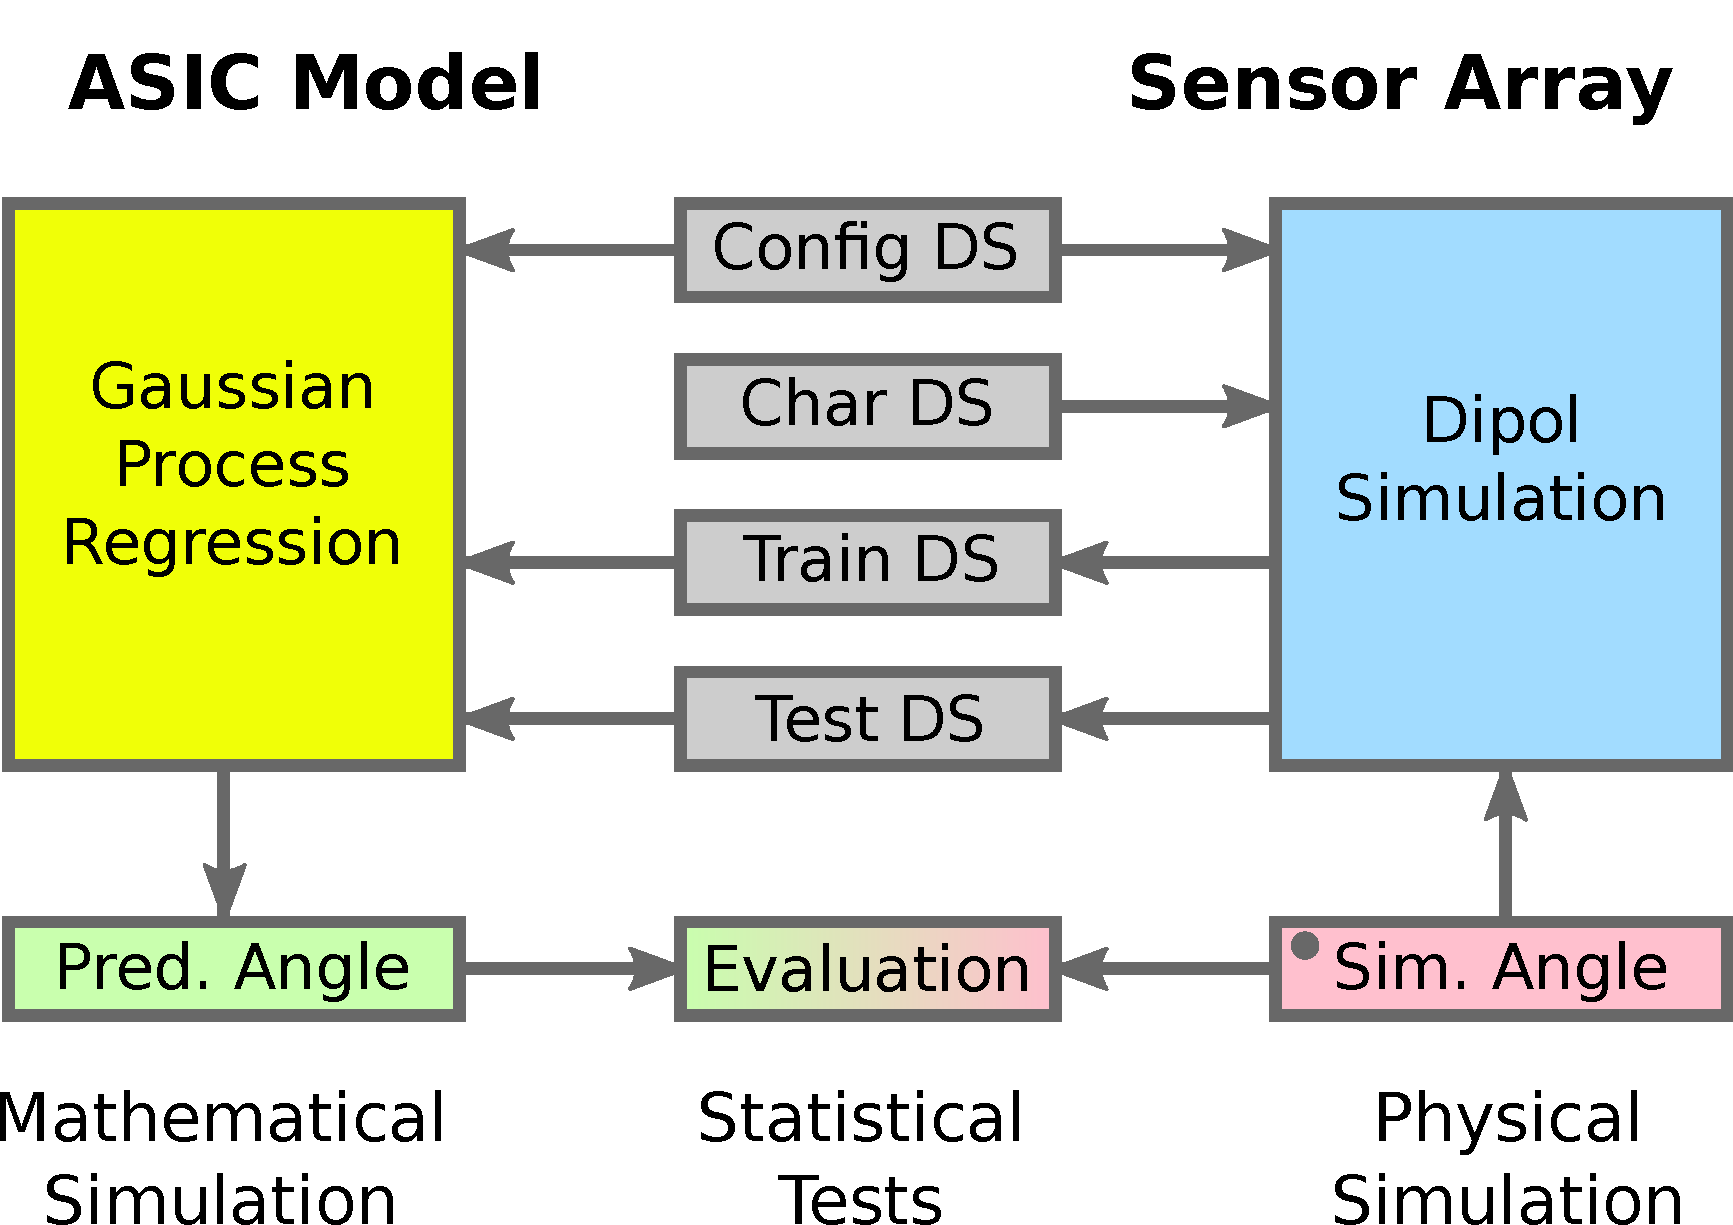
\includegraphics[width=0.7\linewidth]{chapters/images/3-SW-E-OExp/Software-Gesamtansicht}
	\caption[Simulationsaufbau im Überblick]{Simulationsaufbau im Überblick. Konzeptionelle Aufteilung der Simulationen für Sensor-Array und ASIC nach Simulationscharakter. Simulative Kopplung erfolgt, durch prozessierte Datensätze (DS). Eine statistische Auswertung bezieht sich auf angefahrene Simulationswinkel. Der Punkt kennzeichnet die Simulationswinkeleingabe und markiert den gedanklichen Startpunkt des Gesamtkonzepts.}
	\label{fig:software-gesamtansicht}
\end{figure}


Im ersten Simulationsschritt (Sensor-Array) werden Trainings- und Testdatensätze erzeugt. Die Datengenerierung in der Simulation basiert auf Charakterisierungsdatensätze. Diese stellen Technologieeigenschaften und Verhalten für die Simulation bereit, siehe \autoref{ch:tdk-datensatz}. Zur Datengenerierung sind physikalische Gleichungen aus \autoref{sec:sensor-array-simulation-dipol-feldgleichung} genutzt. Als zweiter Simulationsschritt (ASIC-Modell) folgt die Analyse der generierten Daten aus Schritt eins. Zur Analyse wird ein mathematisches Regressionsverfahren verwendet, siehe \autoref{sec:gauss-prozesse-regressionsverfahren}. Das Regressionsverfahren gewichtet Daten und macht entsprechende Vorhersagen gemäß eingestellter Regressionsziele und gewichteten Referenzdaten \autoref{ch:gpr-imp}. Das sind rein mathematische Vorhersagen für vorgegebene Funktionen. Ein physikalischer Gesamtbezug ist durch eine verbundene Auswertung beider Simulationsabschnitte herzustellen. Die Simulationssteuerung ist über einen gemeinsamen Konfigurationsdatensatz umgesetzt, siehe \autoref{tab:sensor-array-sim-params} und \autoref{tab:gpr-sim-params}. Die jeweiligen Parametergruppen sind entsprechend ihrer Zugehörigkeit partiell in den Simulationsbetrieb eingebunden. Der Konfigurationsdatensatz kann je nach Bedarf erzeugt und manipuliert werden. Zur Konfigurationsgenerierung ist das Skript aus \autoref{mcode:generateconfigmat} zu verwenden.


\clearpage


Die Zweischritt-Lösung bietet den Vorteil, dass zuerst verschiedenste Trainings- und Testdatensätze generiert werden können. Nachfolgende und voneinander variierende Simulationen basieren hierbei auf gleichen Datensätzen. Sie sind damit vergleichbar für weitere Auswertungen, Diagnosen oder Optimierungen. Ein empfohlener Arbeitsablauf ist in \autoref{mcode:simulation-workflow} festgehalten.
\newline
Zur Gestaltung der Simulations-Software ist ein modularer Ansatz nach \autoref{fig:blockschemasoftware} verfolgt worden. Das modulare Konzept erhöht die Wiederverwendbarkeit des Quellcodes. Es ermöglicht einzelne Quellcodebestandteile miteinander zu kombinieren. Die Einbindung und Ausführung der Quellcodemodule aus \autoref{mcode:source-code} erfolgt in Skripten des \autoref{mcode:executable-scripts}. Die Software ist als Projekt in der Multi-Paradigmen-Programmiersprache Matlab umgesetzt, siehe \autoref{ch:genutzte-sw}. Konzeptrichtlinien sind im \autoref{mcode:workflows} festgehalten. Zusätzliche Anweisungen zur Arbeitsweise, Projektpflege, Dokumentation und Vorlagen für Skripte und Funktionen sind beigefügt. Alle Entwicklungsschritte sind mittels Git-Versionsverwaltung kommentiert und nachvollziehbar dokumentiert. Jede Quellcode- und Skript-Datei ist nach festgelegten Konventionen geschrieben worden \cite{Johnson2014}. Es ermöglicht eine automatisierte Dokumentation des gesamten Software-Projekts in \autoref{ch:sw-doku}. Erzeugt ist diese mit Skripten aus \autoref{mcode:publishprojectfilestohtml} und \autoref{mcode:exportpublishedtopdf}.


\vspace{3mm}
\begin{figure}[bph]
	\centering
	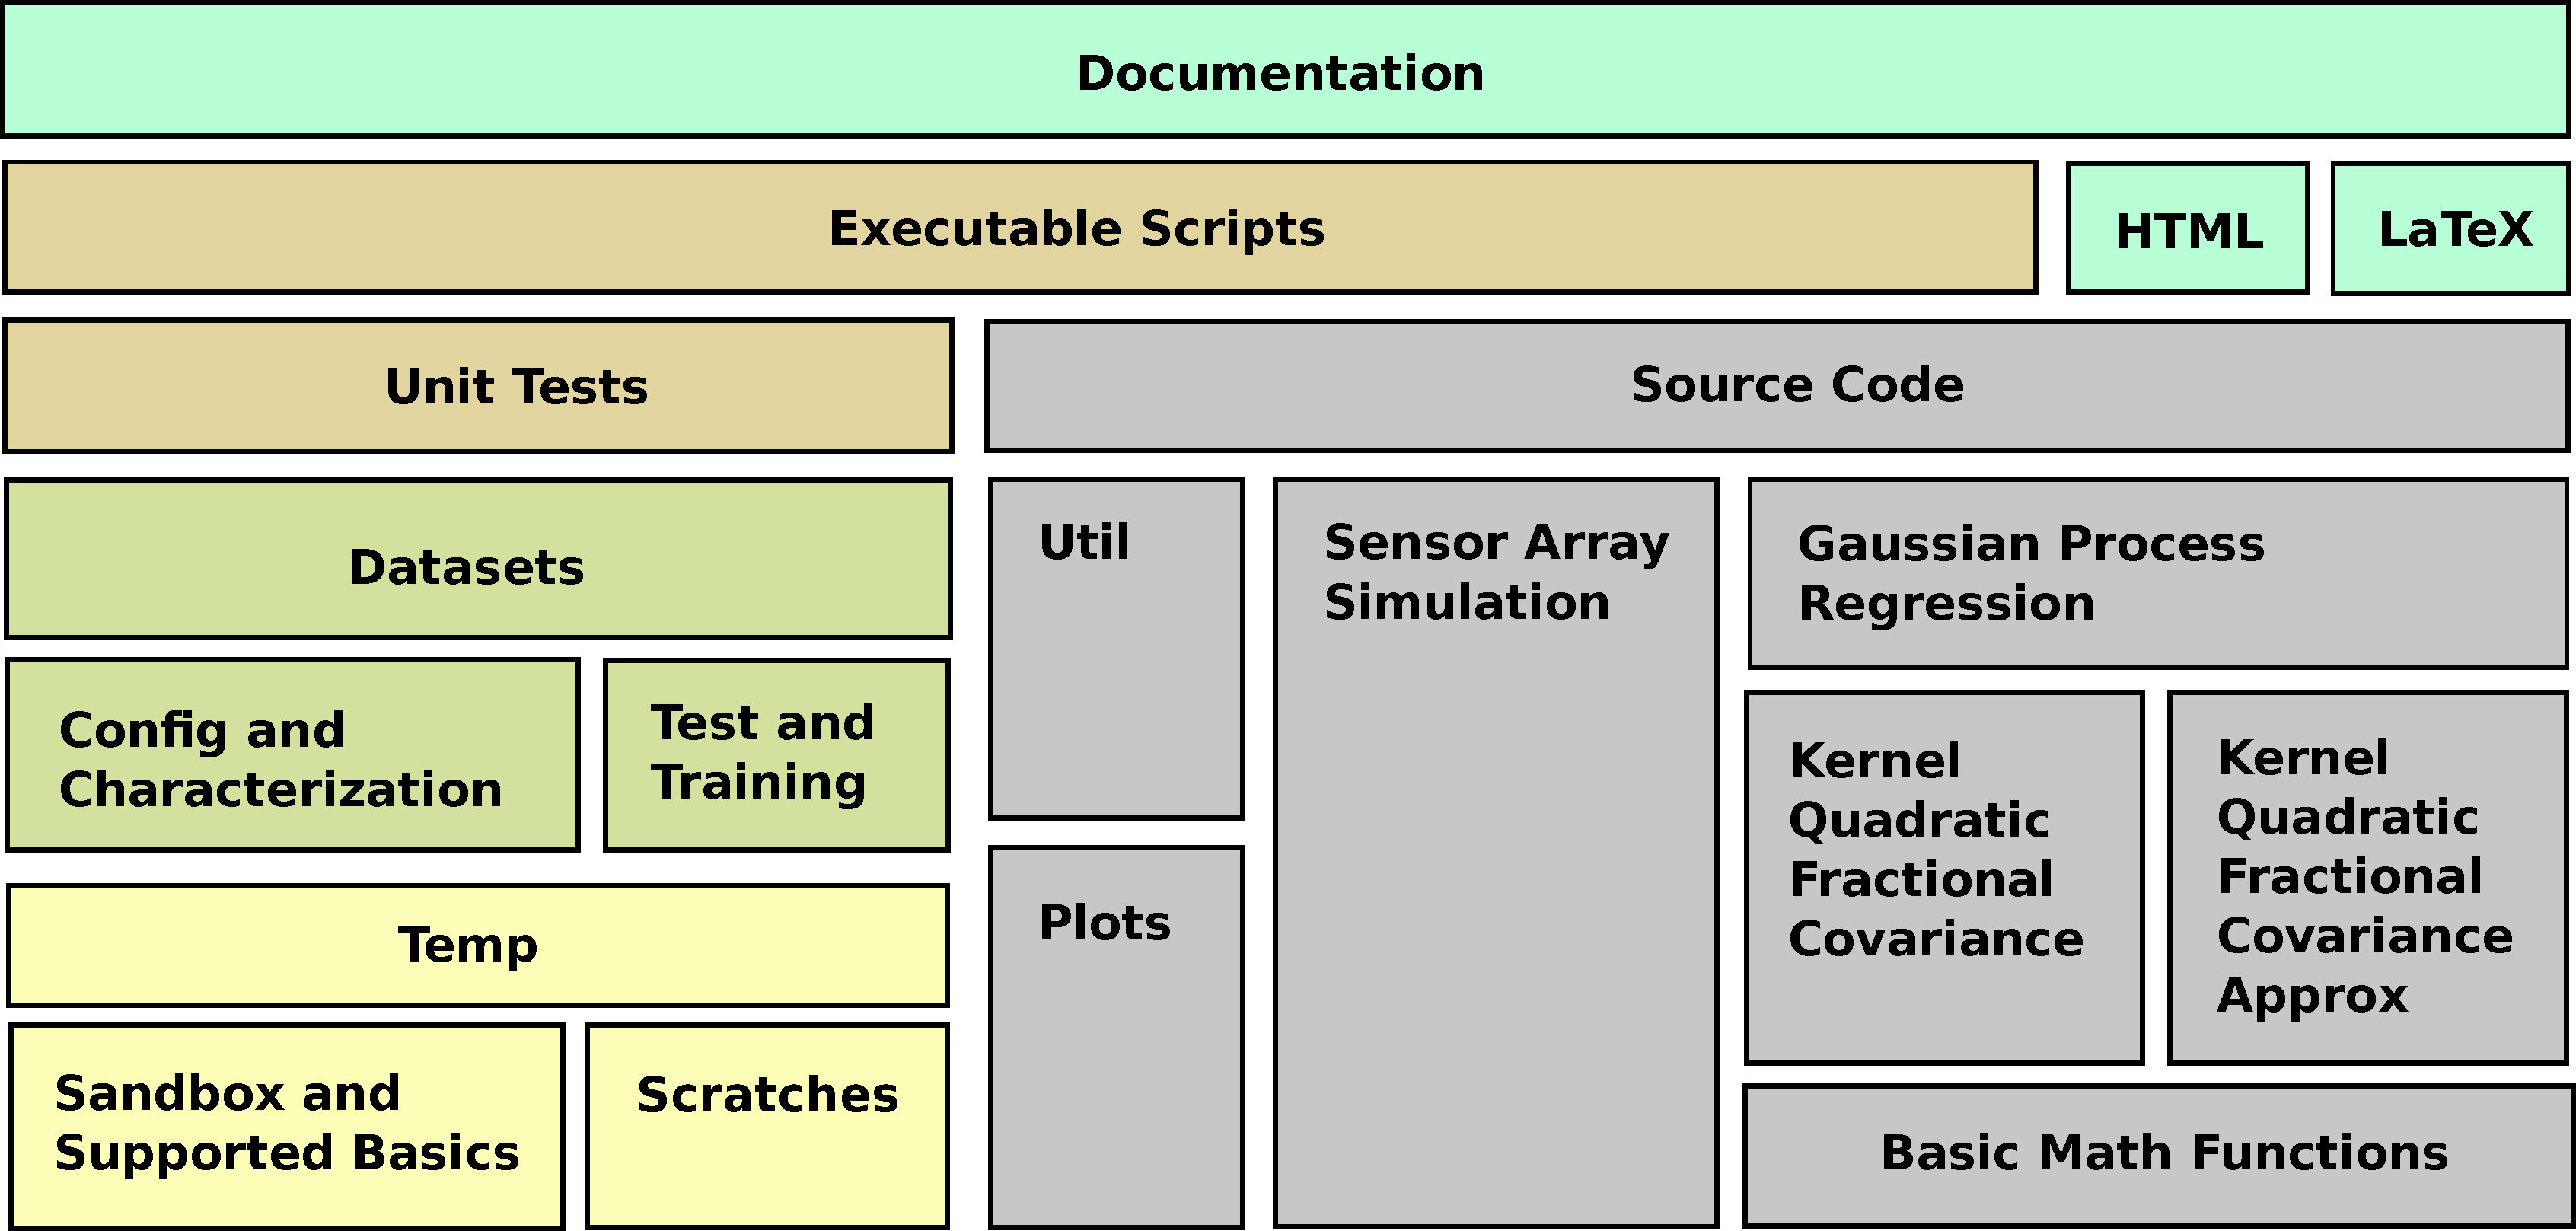
\includegraphics[width=\linewidth]{chapters/images/3-SW-E-OExp/Blockschema_Software}
	\caption[Blockschema Simulations-Software]{Blockschema Simulations-Software. Modulare Software-Gestaltung. Kernbestandteil ist funktionaler Quellcode. Quellcodemodule sind mit Datensätzen nach Bedarf in Skripten zu laden und ausführbar. Software-Dokumentation steht in HTML und LaTeX bereit. Als HTML ist diese in Matlab integriert. Entwurfsarbeiten sind nicht Bestandteil der Dokumentation, aber im Projektverzeichnis vorliegend.}
	\label{fig:blockschemasoftware}
\end{figure}


\clearpage

% !TEX root = ../thesis.tex
% simulation processes and execution
% @author Tobias Wulf
%

\section{Simulationsprozesse und Ausführung}\label{sec:sim-pro}


\subsection{Sensor-Array-Simulation}\label{sub:sensor-array-pro}


\begin{figure}[tbph]
	\centering
	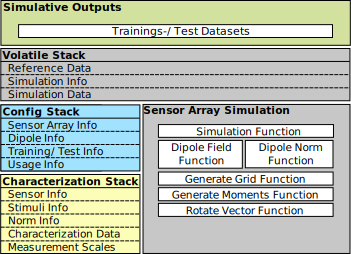
\includegraphics[width=0.7\linewidth]{chapters/images/3-SW-E-OExp/Blockschema_Sensor-Array}
	\caption[Blockschema Einbindung der Sensor-Array-Simulation]{Blockschema Einbindung der Sensor-Array-Simulation}
	\label{fig:blockschemasensor-array}
\end{figure}


\clearpage


\begin{figure}[tbph]
	\centering
	\includegraphics[width=\linewidth]{chapters/images/3-SW-E-OExp/Sensor-Array-Simulation}
	\caption[Sensor-Array-Simulation Prozessansicht]{Sensor-Array-Simulation Prozessansicht}
	\label{fig:sensor-array-simulation}
\end{figure}


\clearpage


\subsection{Gauß-Prozess-Regression}\label{sub:gpr-pro}


\paragraph{Trainingsphase}\label{par:gpr-training-pro}$~$\\


\begin{figure}[tbph]
	\centering
	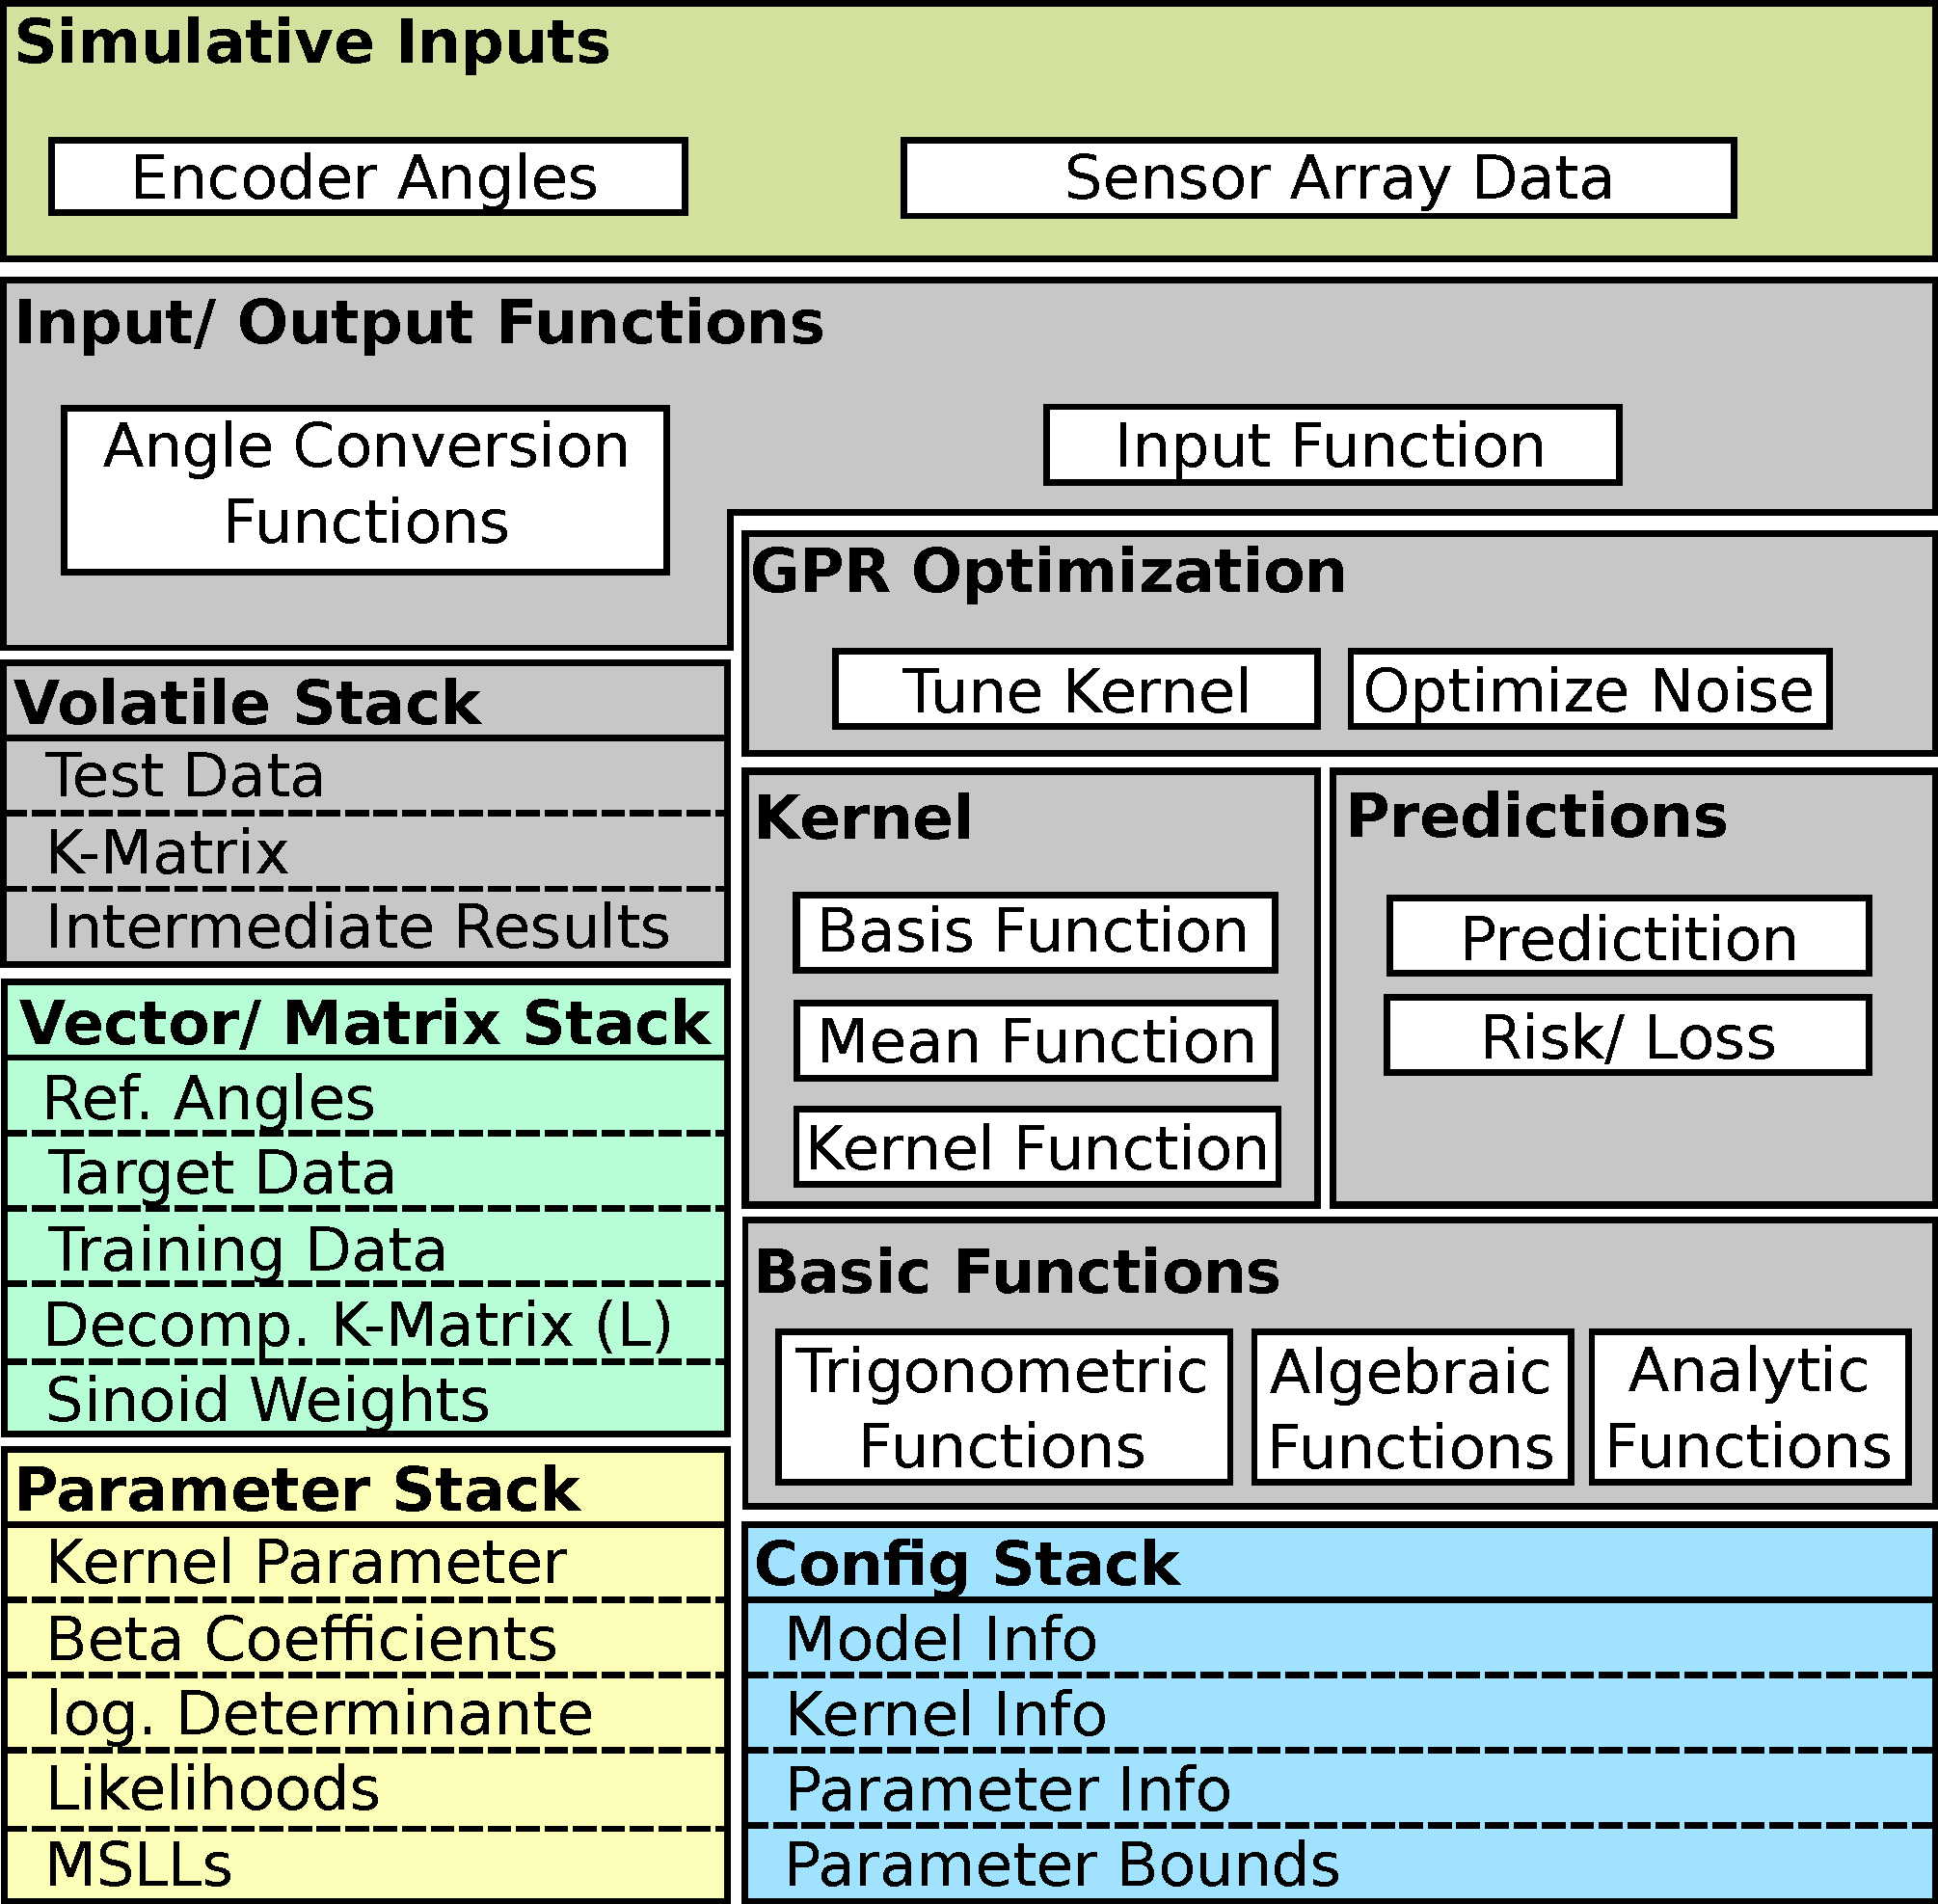
\includegraphics[width=0.7\linewidth]{chapters/images/3-SW-E-OExp/Blockschema_Trainingsphase}
	\caption[Blockschema Trainingsphase Regression]{Blockschema Trainingsphase Regression}
	\label{fig:blockschematrainingsphase}
\end{figure}


\clearpage


\begin{figure}[tbph]
	\centering
	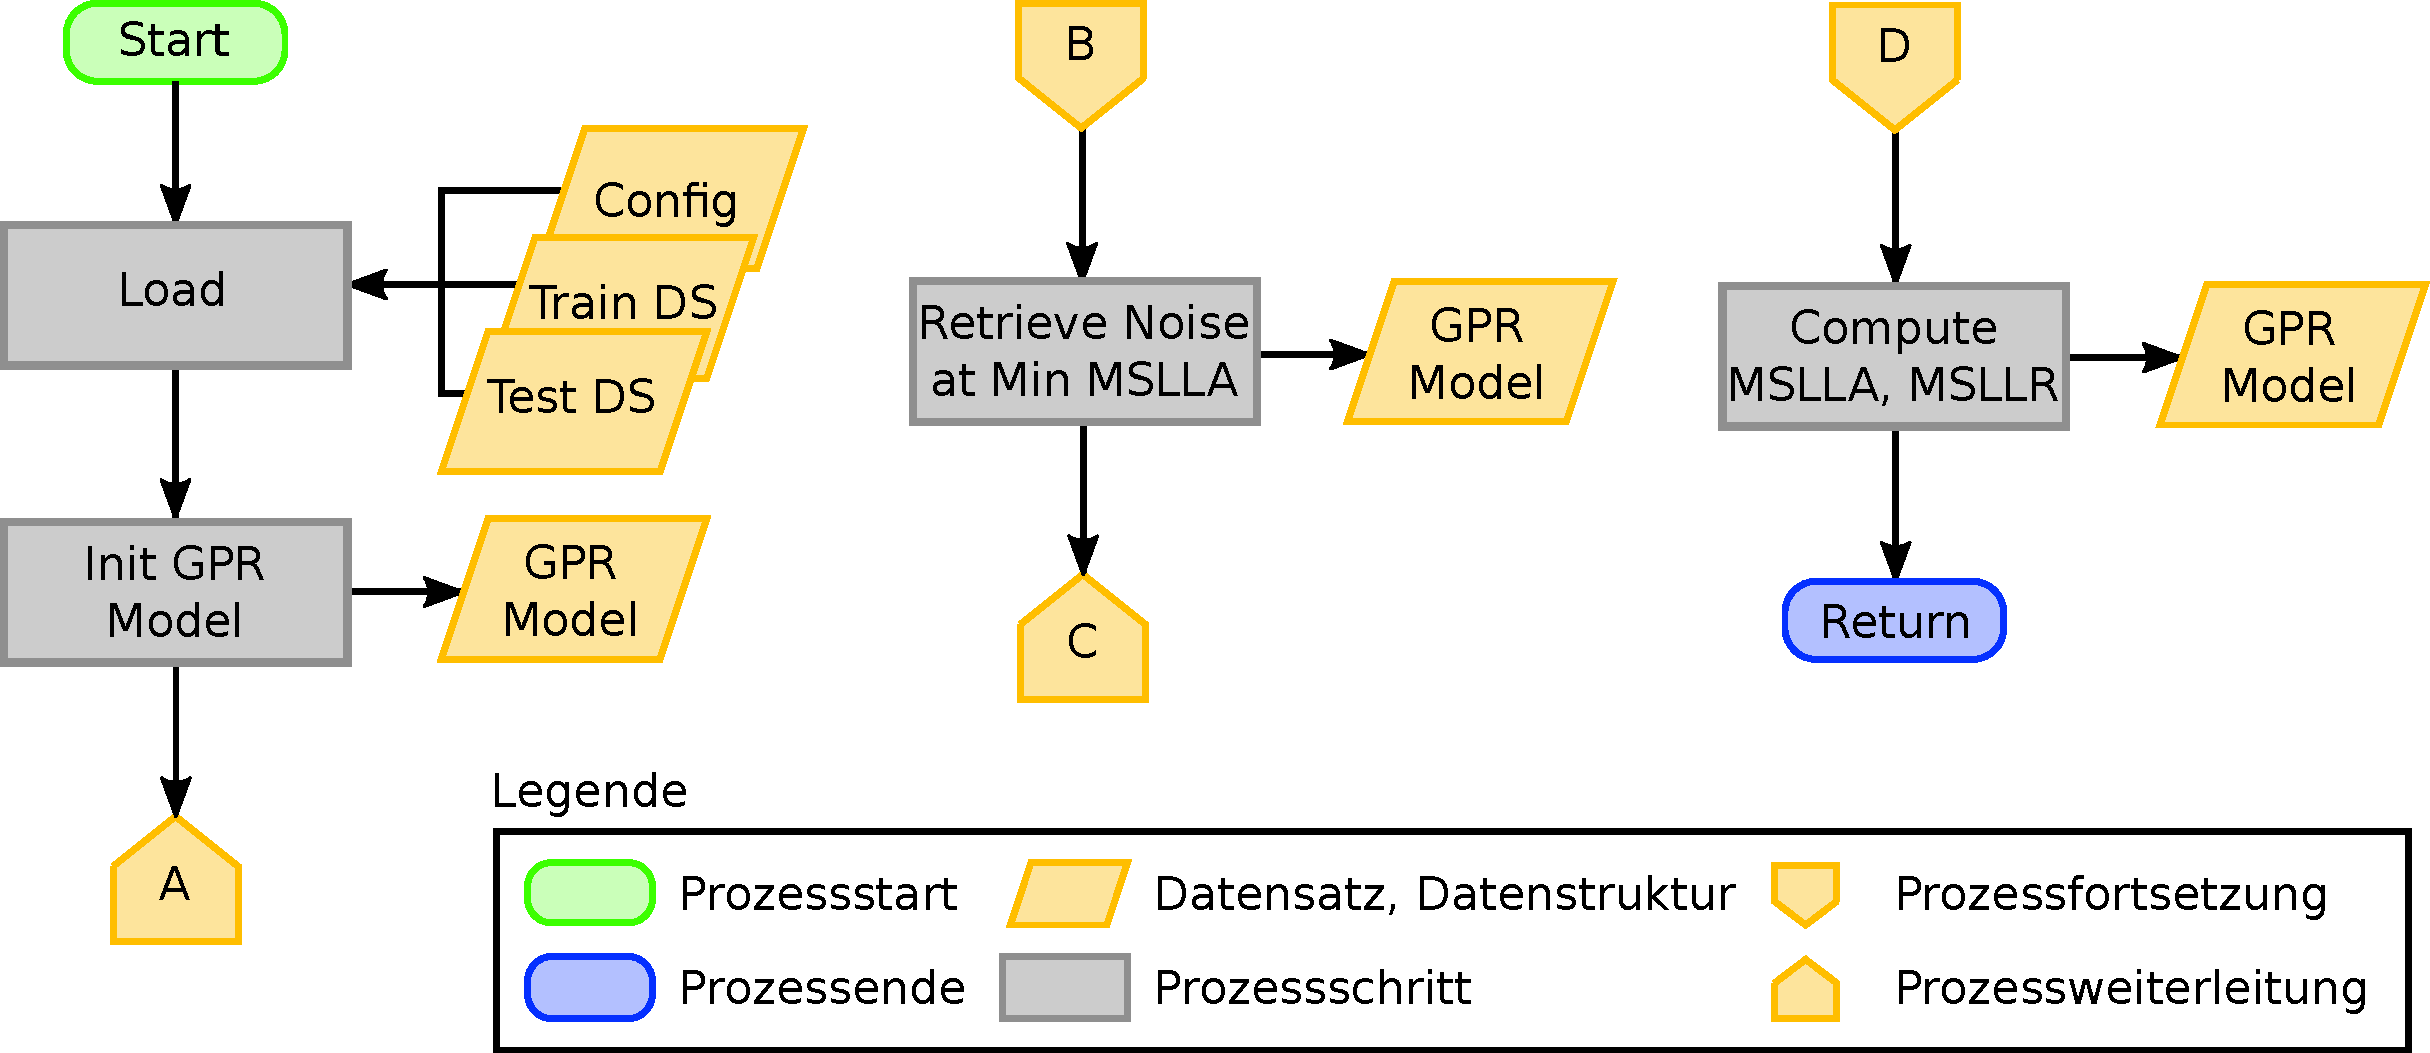
\includegraphics[width=.8\linewidth]{chapters/images/3-SW-E-OExp/GPR_Optimization}
	\caption[Regressionsoptimierung/ -Generalisierung Prozessansicht]{Regressionsoptimierung/ -Generalisierung Prozessansicht}
	\label{fig:gproptimization}
\end{figure}


\clearpage


\begin{figure}[htbp]
	\centering
	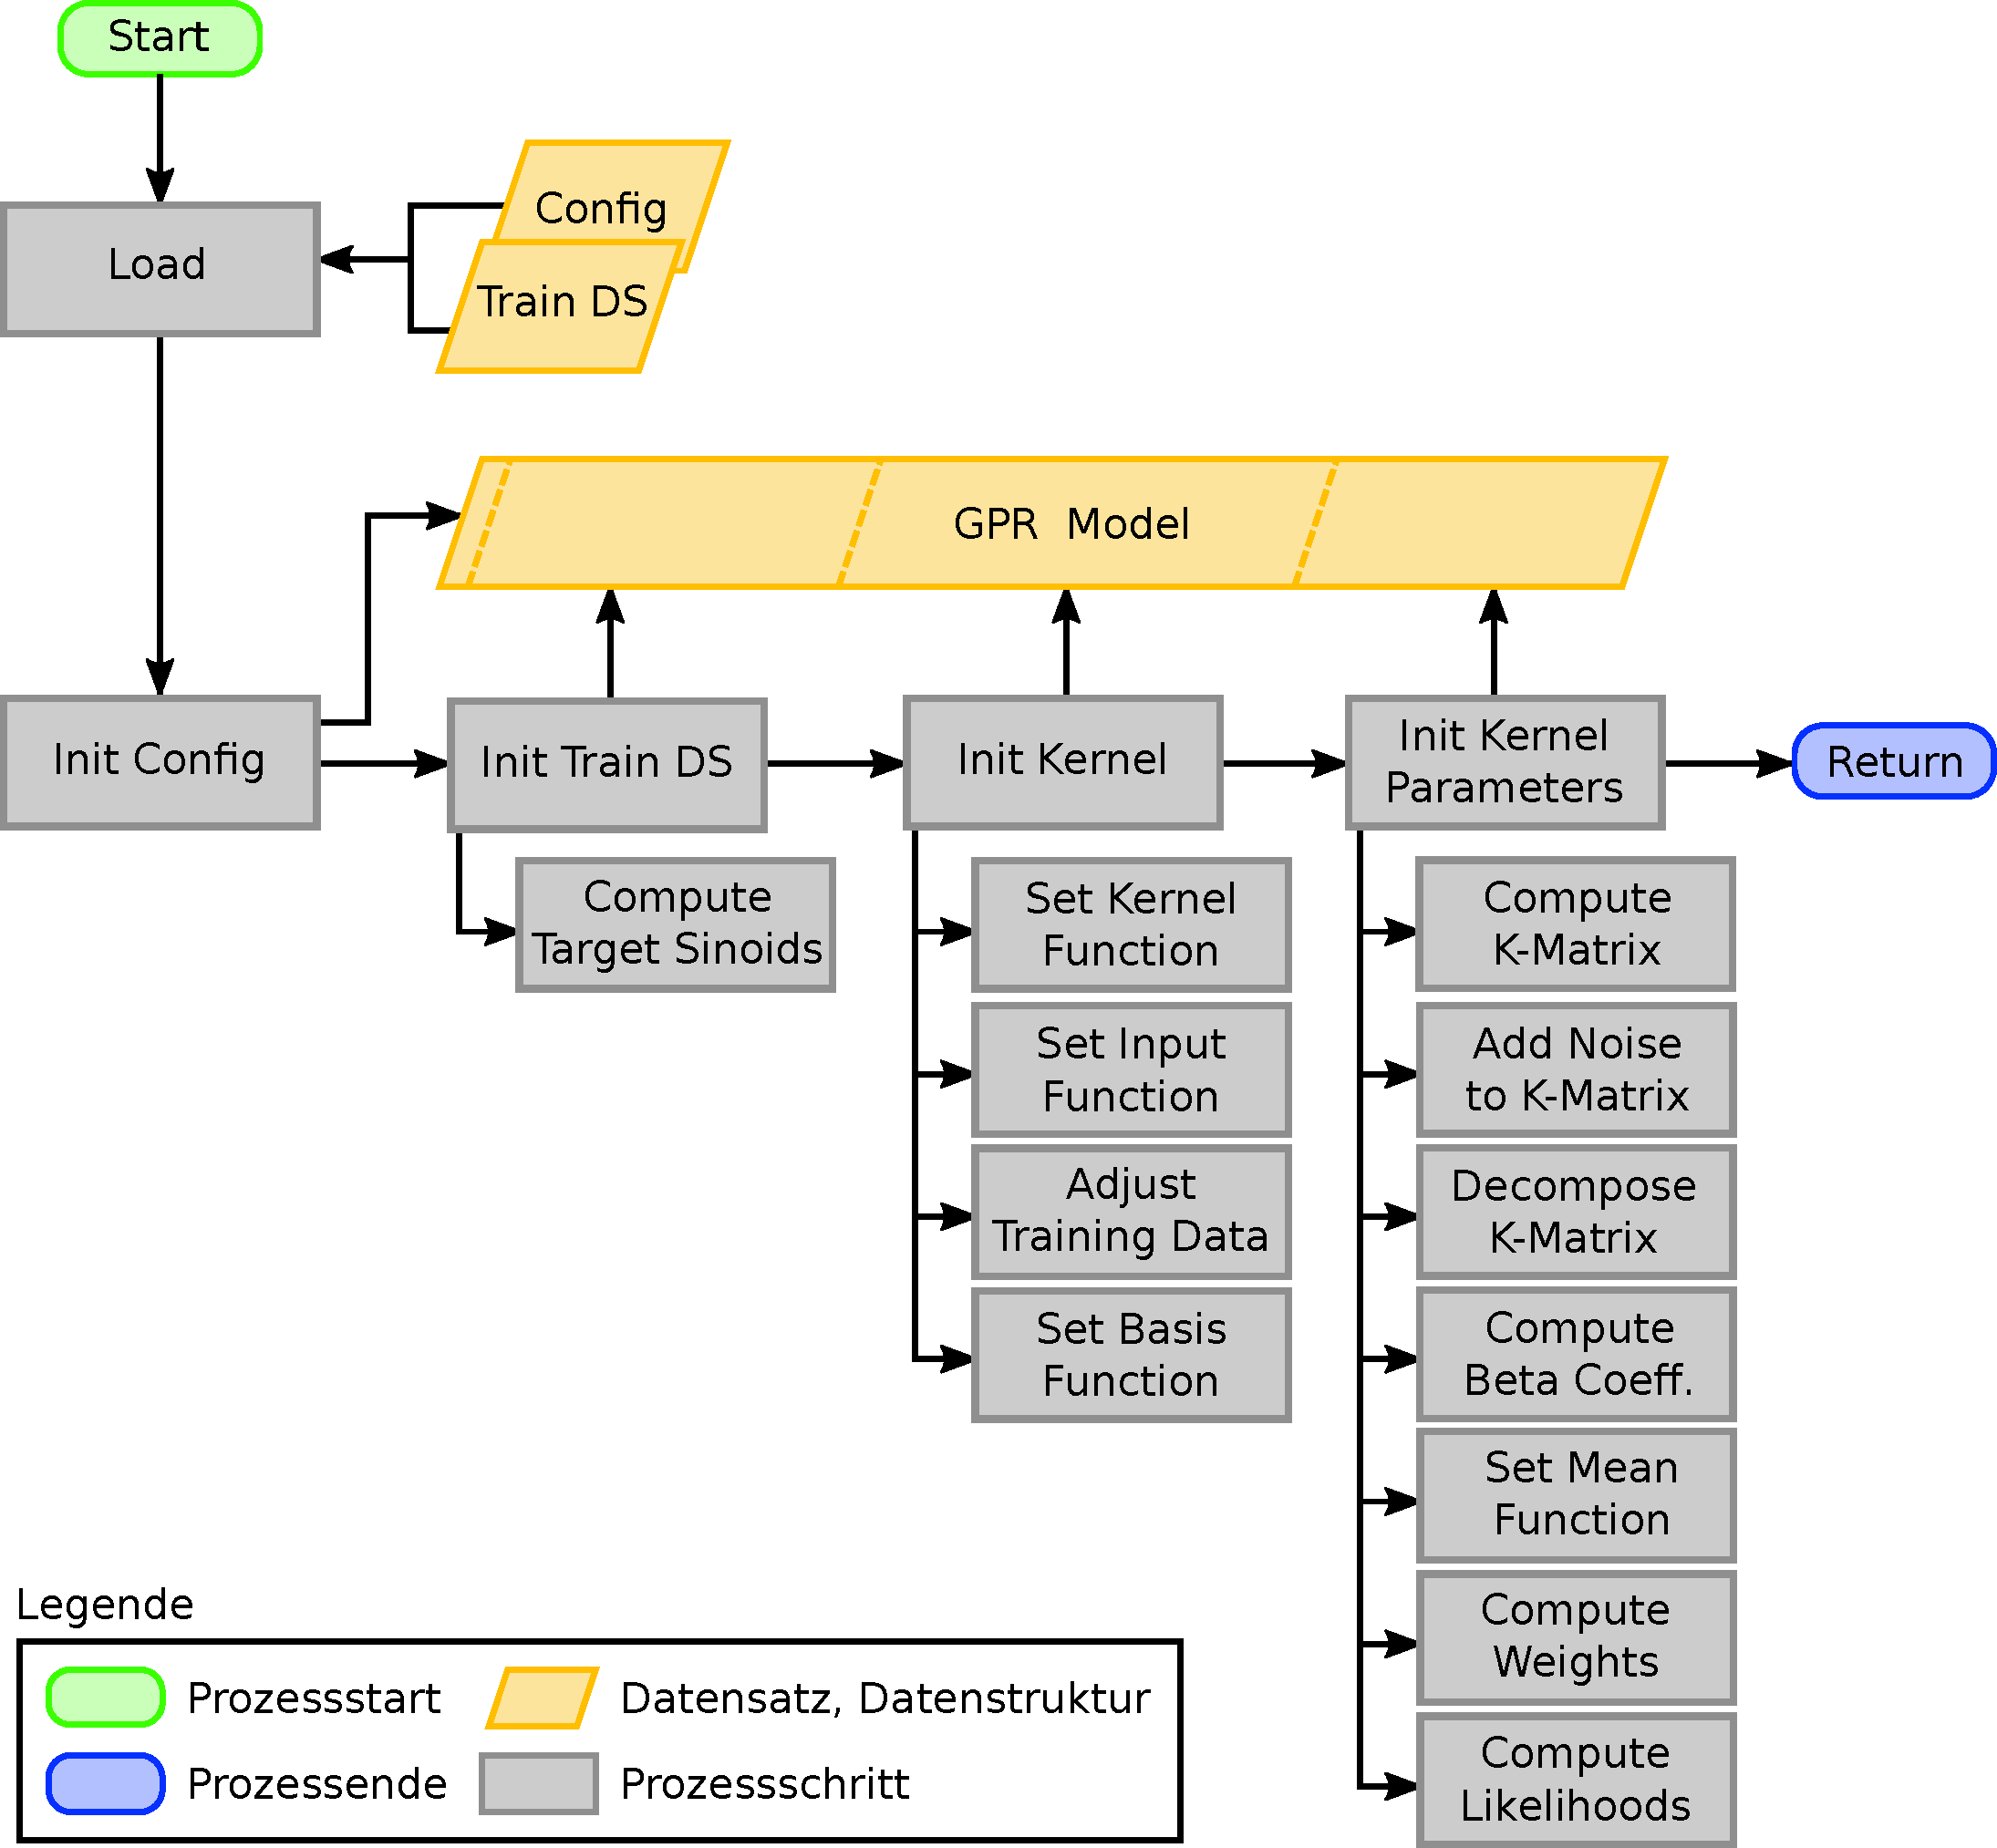
\includegraphics[width=0.7\linewidth]{chapters/images/3-SW-E-OExp/GPR_Initialization}
	\caption[Regressionsinitialisierung Prozessansicht]{Regressionsinitialisierung Prozessansicht}
	\label{fig:gprinitialization}
\end{figure}


\clearpage


\begin{figure}[tbph]
	\centering
	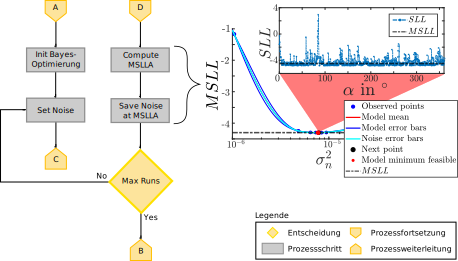
\includegraphics[width=0.85\linewidth]{chapters/images/3-SW-E-OExp/Noise_Optimization}
	\caption[Rauschniveauoptimierung Prozessansicht]{Rauschniveauoptimierung Prozessansicht}
	\label{fig:noiseoptimization}
\end{figure}


\clearpage


\begin{figure}[tbph]
	\centering
	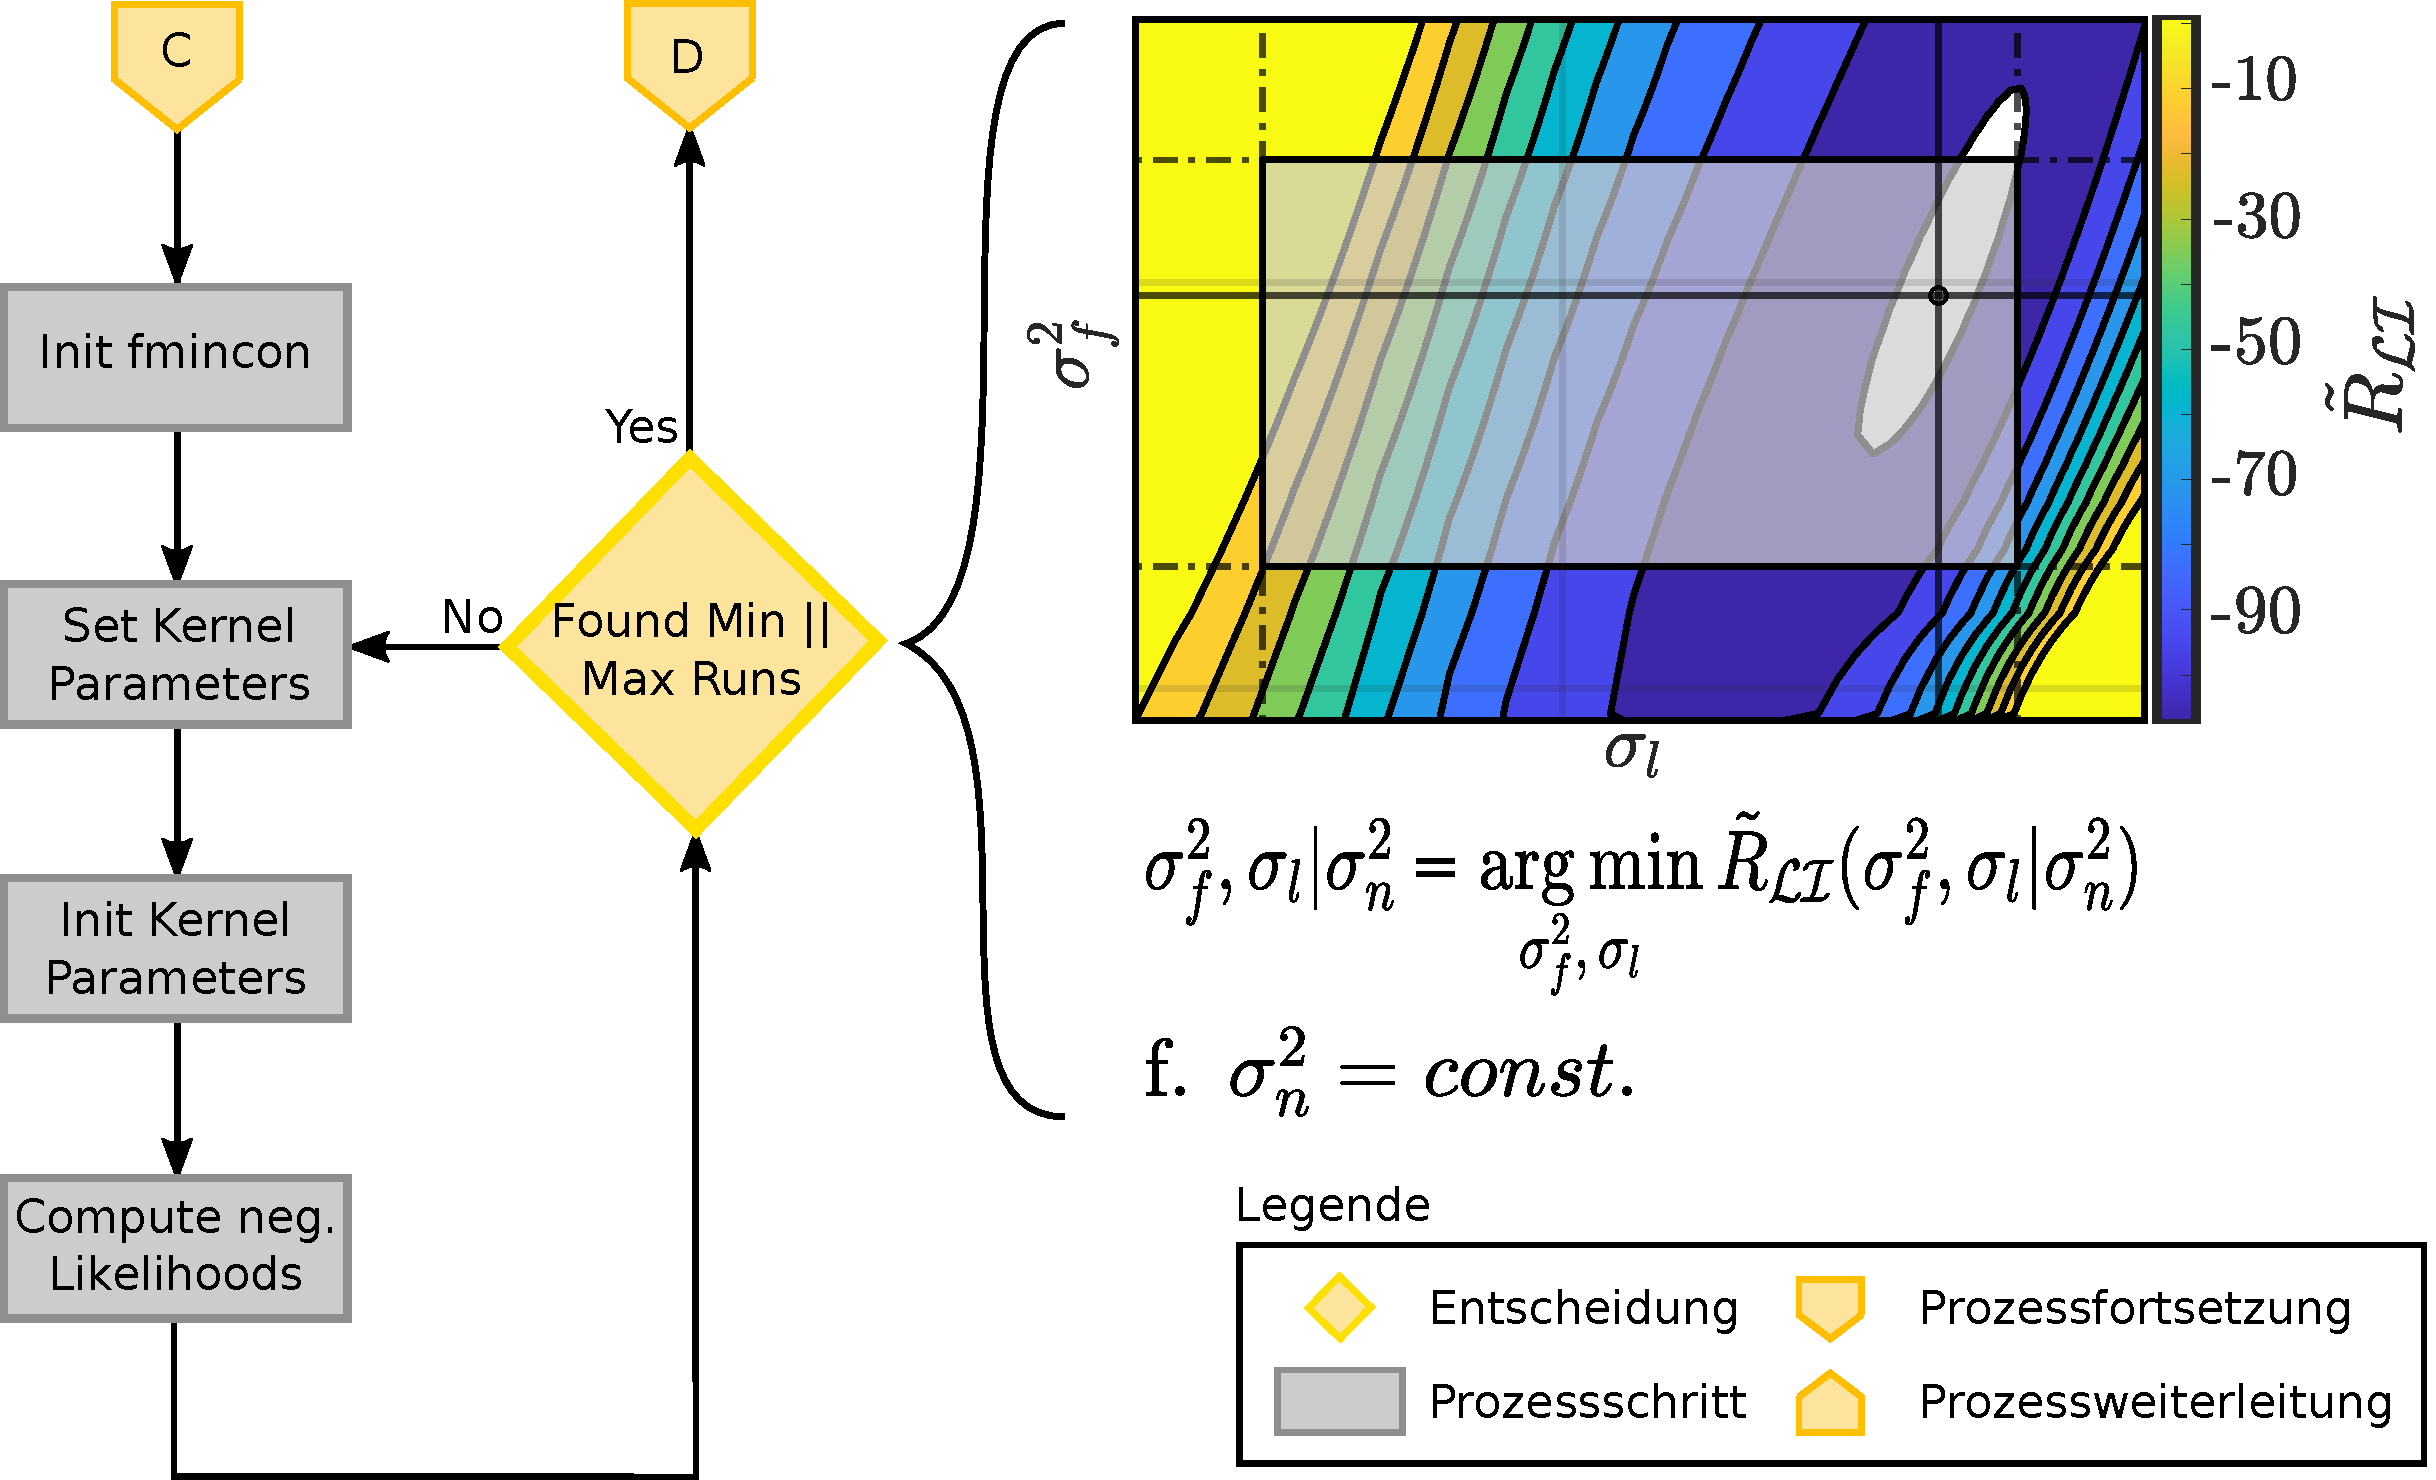
\includegraphics[width=0.8\linewidth]{chapters/images/3-SW-E-OExp/Kernel_Tuning}
	\caption[Regressionsparameteroptimierung Prozessansicht]{Regressionsparameteroptimierung Prozessansicht}
	\label{fig:kerneltuning}
\end{figure}


\clearpage


\paragraph{Arbeitsphase}\label{par:gpr-work-pro}$~$\\


\begin{figure}[tbph]
	\centering
	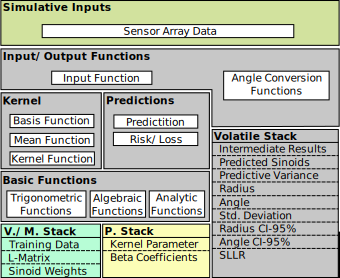
\includegraphics[width=0.7\linewidth]{chapters/images/3-SW-E-OExp/Blockschema_Workphase}
	\caption[Blockschema Arbeitsphase Regression]{Blockschema Arbeitsphase Regression}
	\label{fig:blockschemaworkphase}
\end{figure}

